\documentclass[../document.tex]{subfiles}
\begin{document}\label{ssec:time}

\captionsetup[subfigure]{justification=raggedright,singlelinecheck=false}

\begin{figure*}
	\begin{subfigure}{0.09\textwidth}\subcaption[l]{\bf kmeans} \label{fig:time-kmeans} \vspace{5mm}\end{subfigure}
	\begin{subfigure}{0.9\textwidth}
		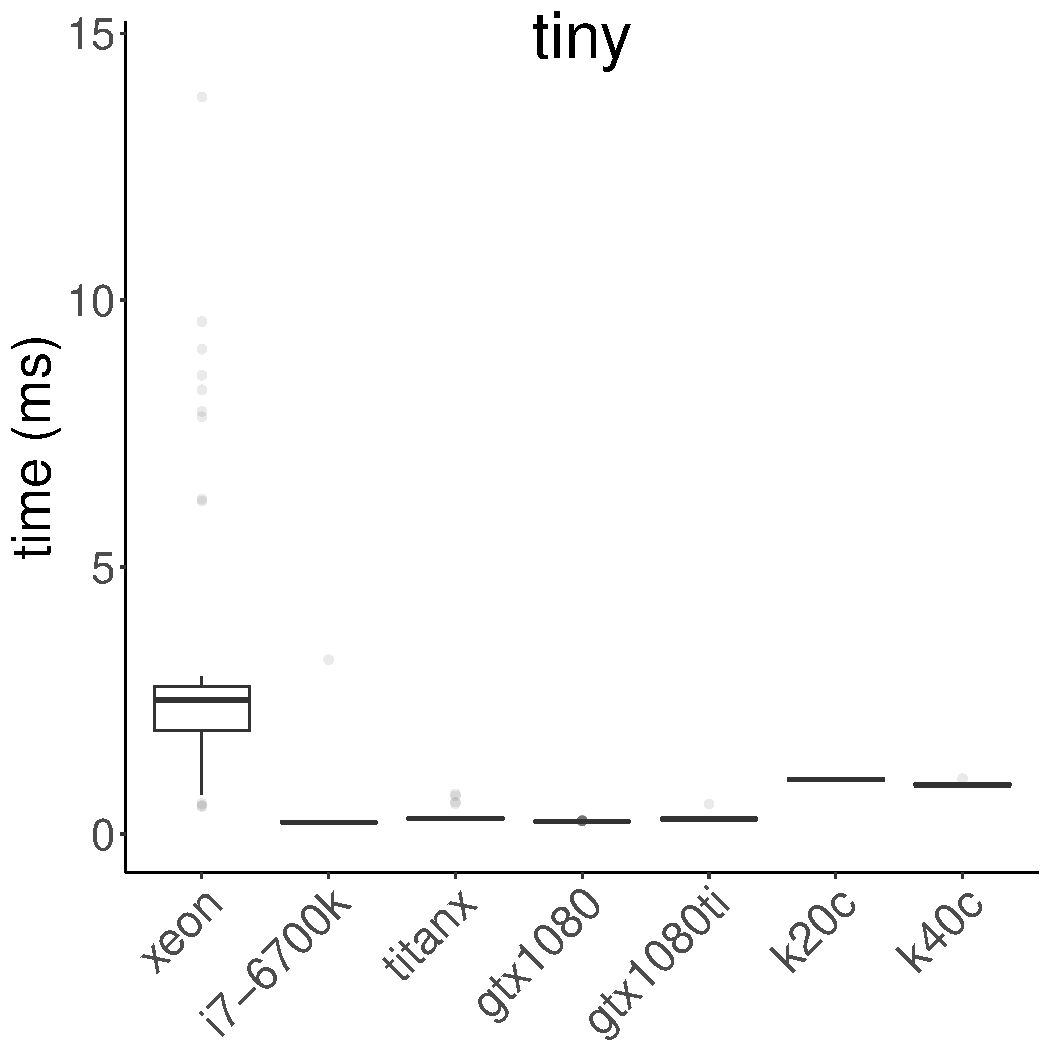
\includegraphics[width=0.22\textwidth]{figures/time-results/generate_kmeans_no_knl_tiny_boxplot-1}
		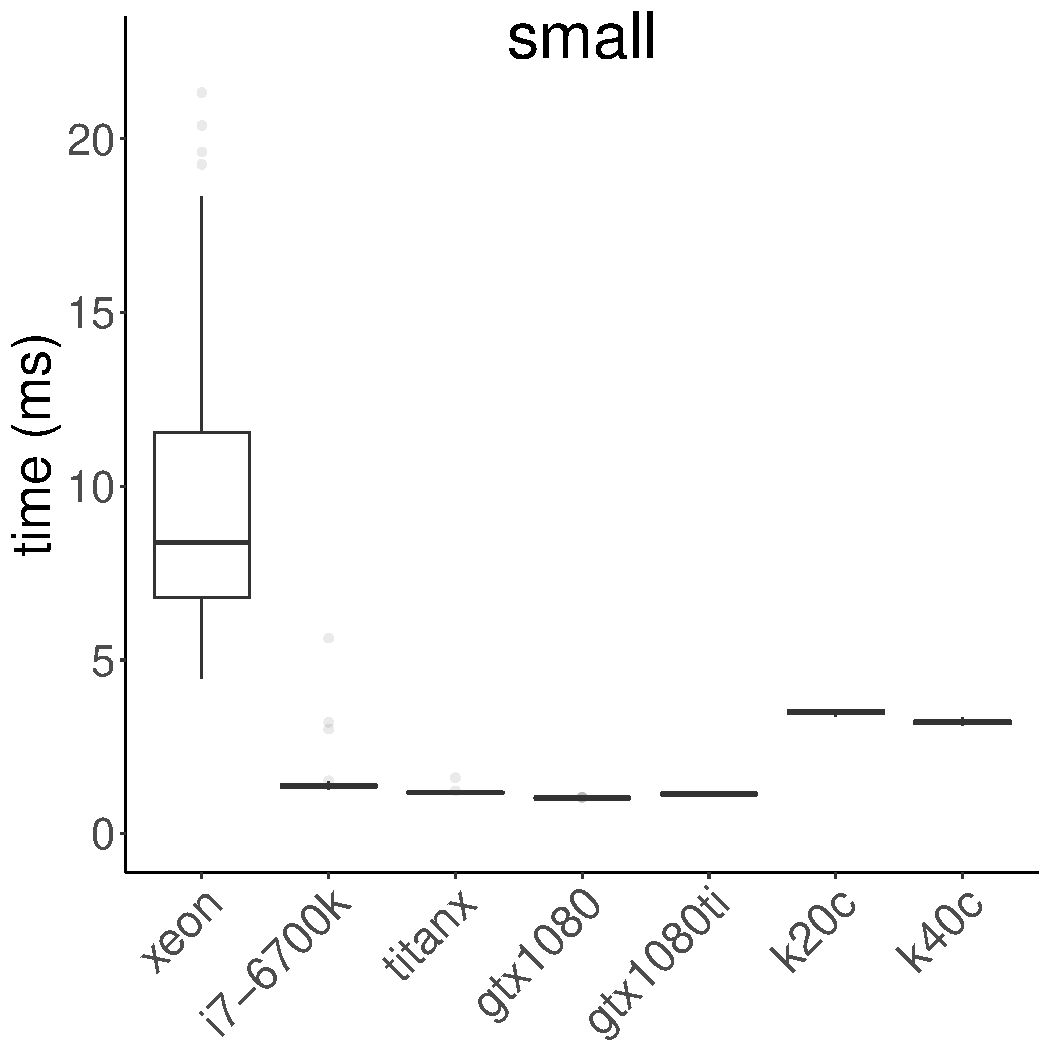
\includegraphics[width=0.22\textwidth]{figures/time-results/generate_kmeans_no_knl_small_boxplot-1}
		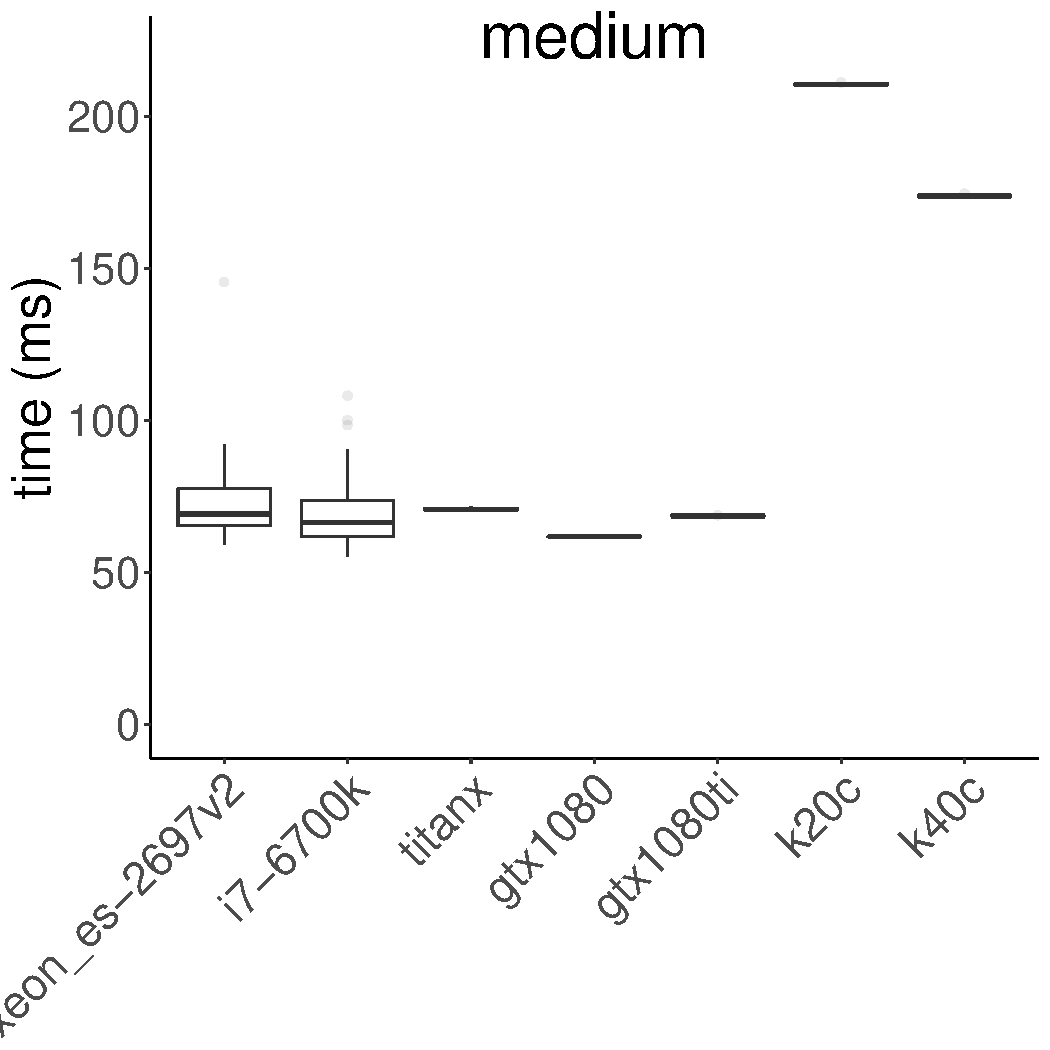
\includegraphics[width=0.22\textwidth]{figures/time-results/generate_kmeans_no_knl_medium_boxplot-1}
		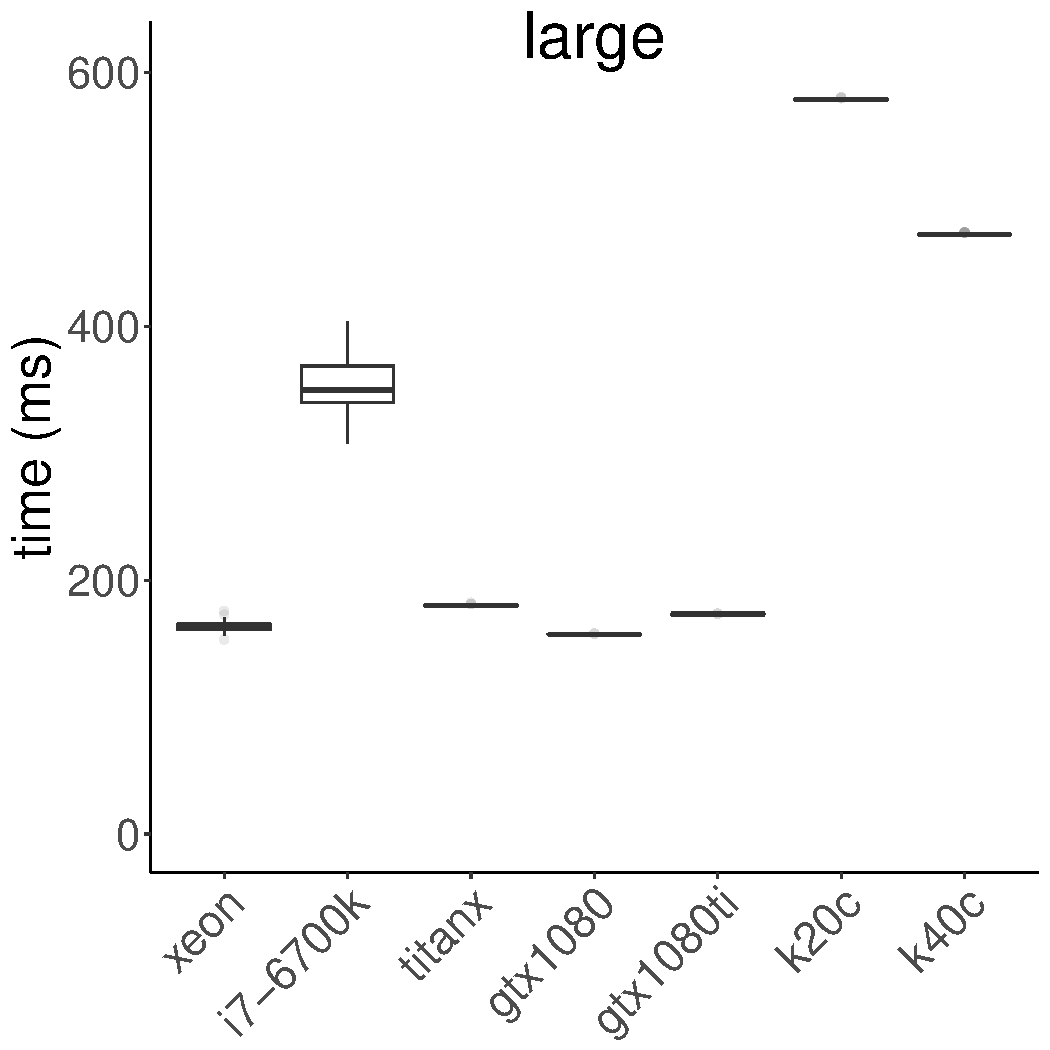
\includegraphics[width=0.22\textwidth]{figures/time-results/generate_kmeans_no_knl_large_boxplot-1}
	\end{subfigure}

	\begin{subfigure}{0.09\textwidth}\subcaption[l]{\bf lud} \label{fig:time-lud} \vspace{5mm}\end{subfigure}
	\begin{subfigure}{0.9\textwidth}
		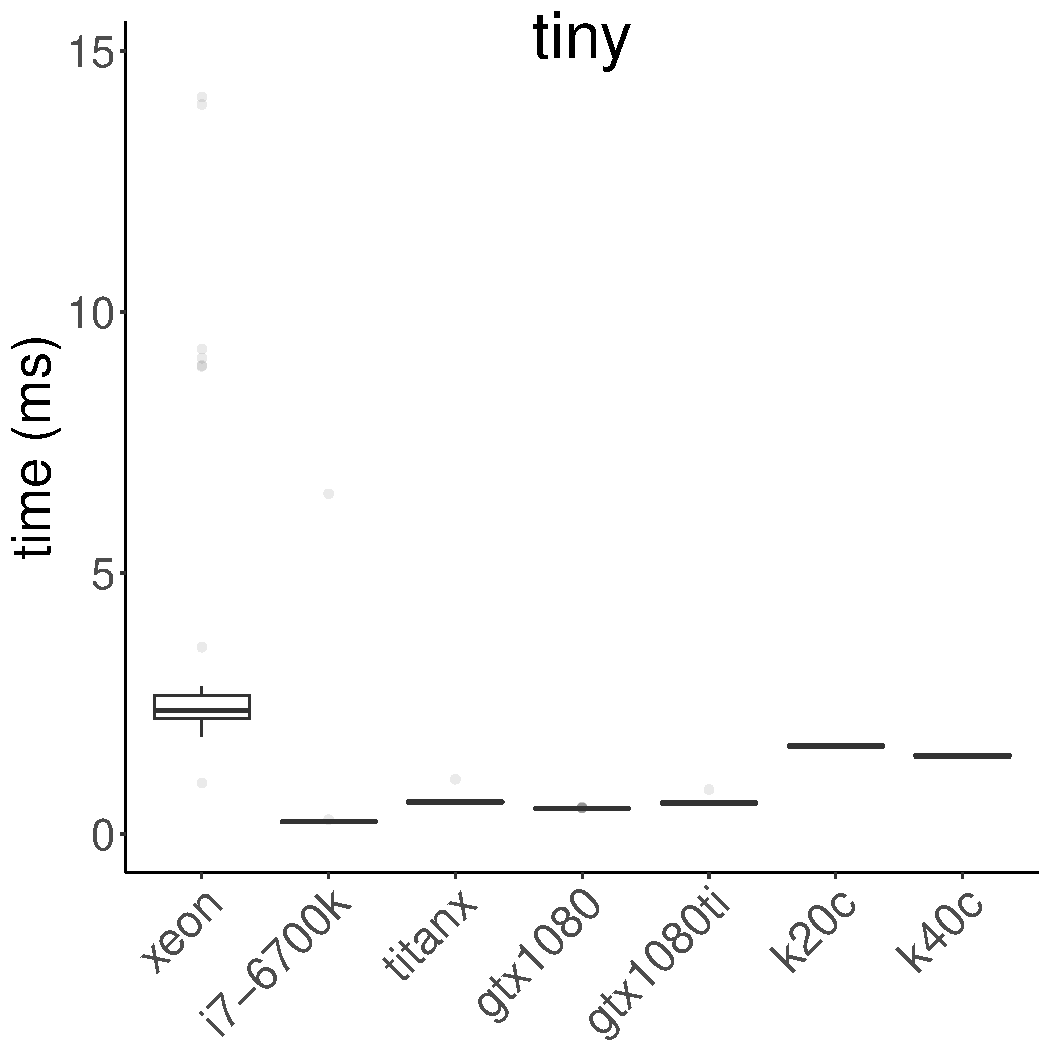
\includegraphics[width=0.22\textwidth]{figures/time-results/generate_lud_tiny_boxplot-1}
		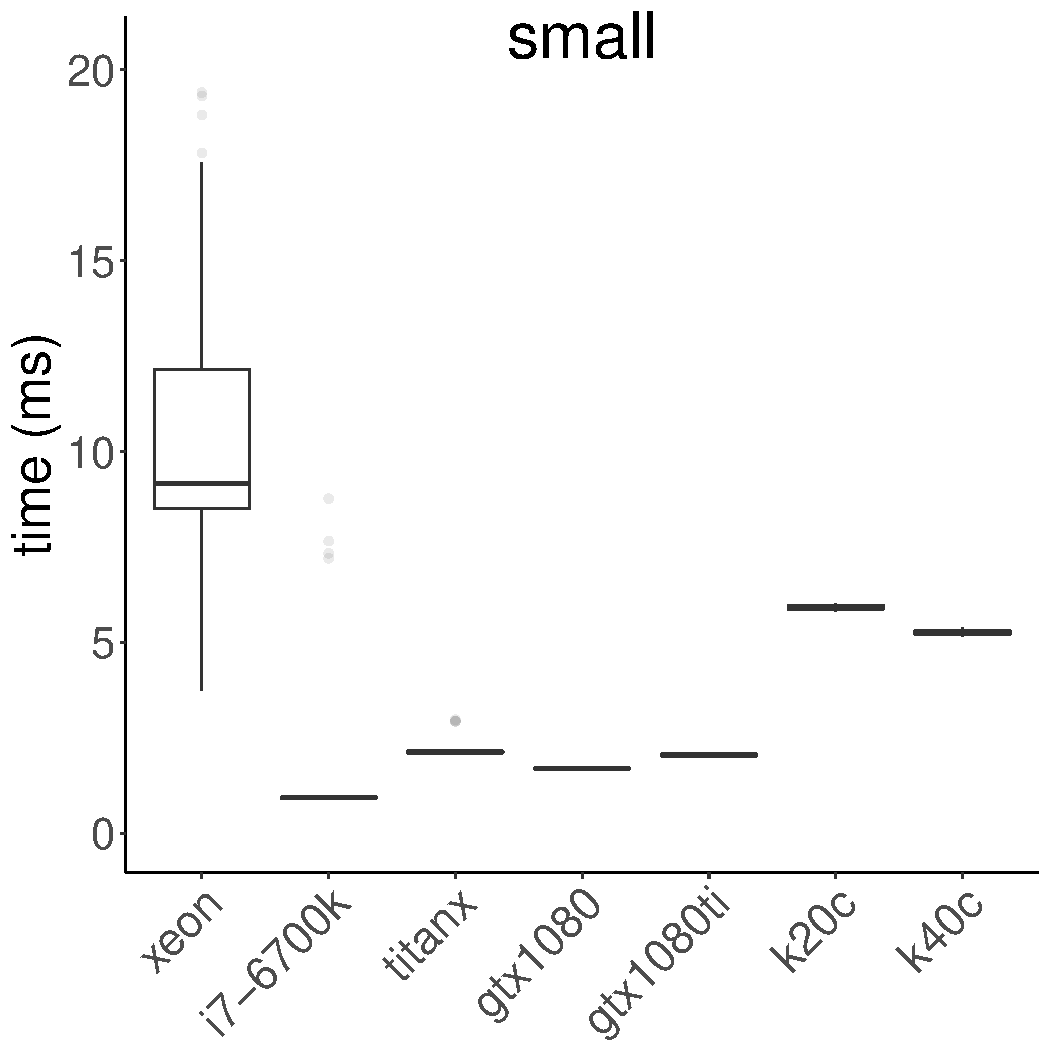
\includegraphics[width=0.22\textwidth]{figures/time-results/generate_lud_small_boxplot-1}
		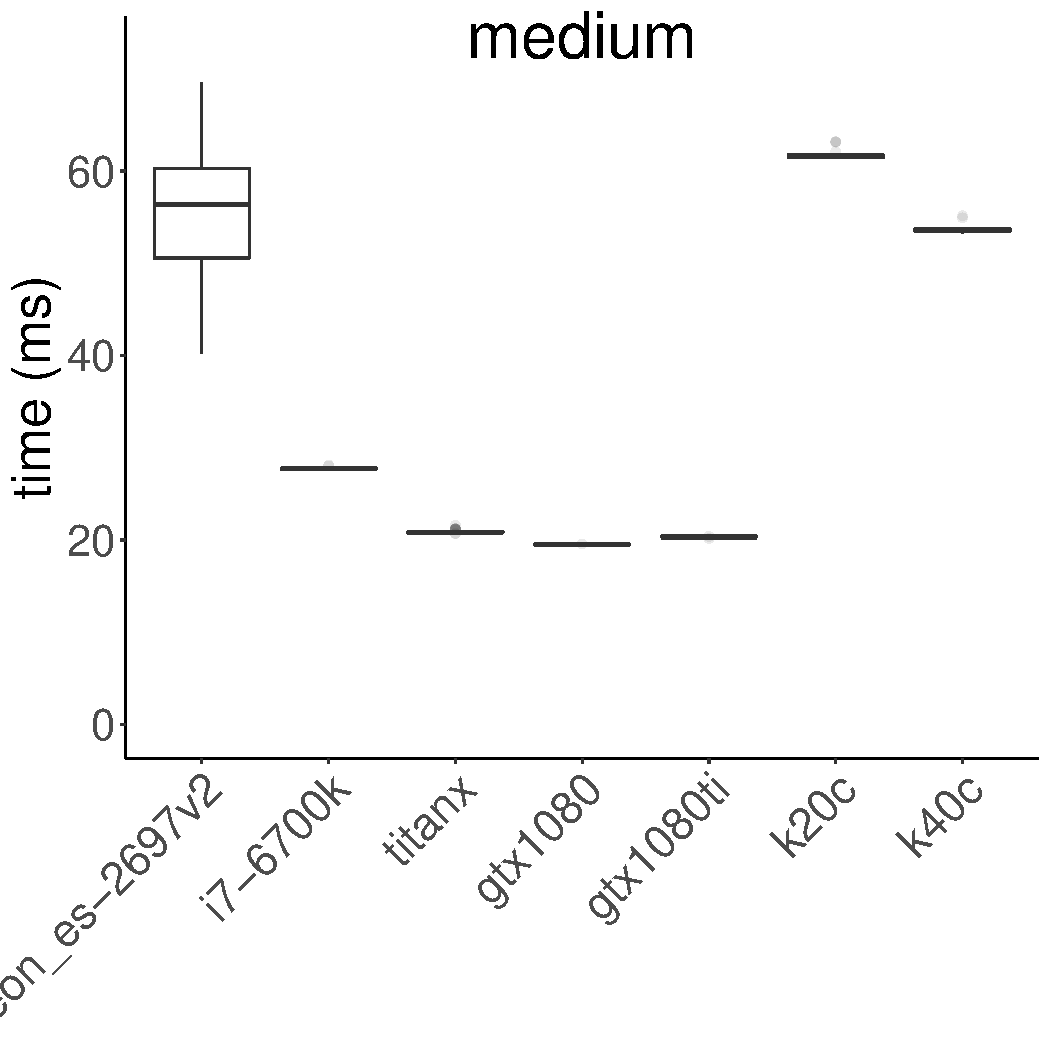
\includegraphics[width=0.22\textwidth]{figures/time-results/generate_lud_medium_boxplot-1}
		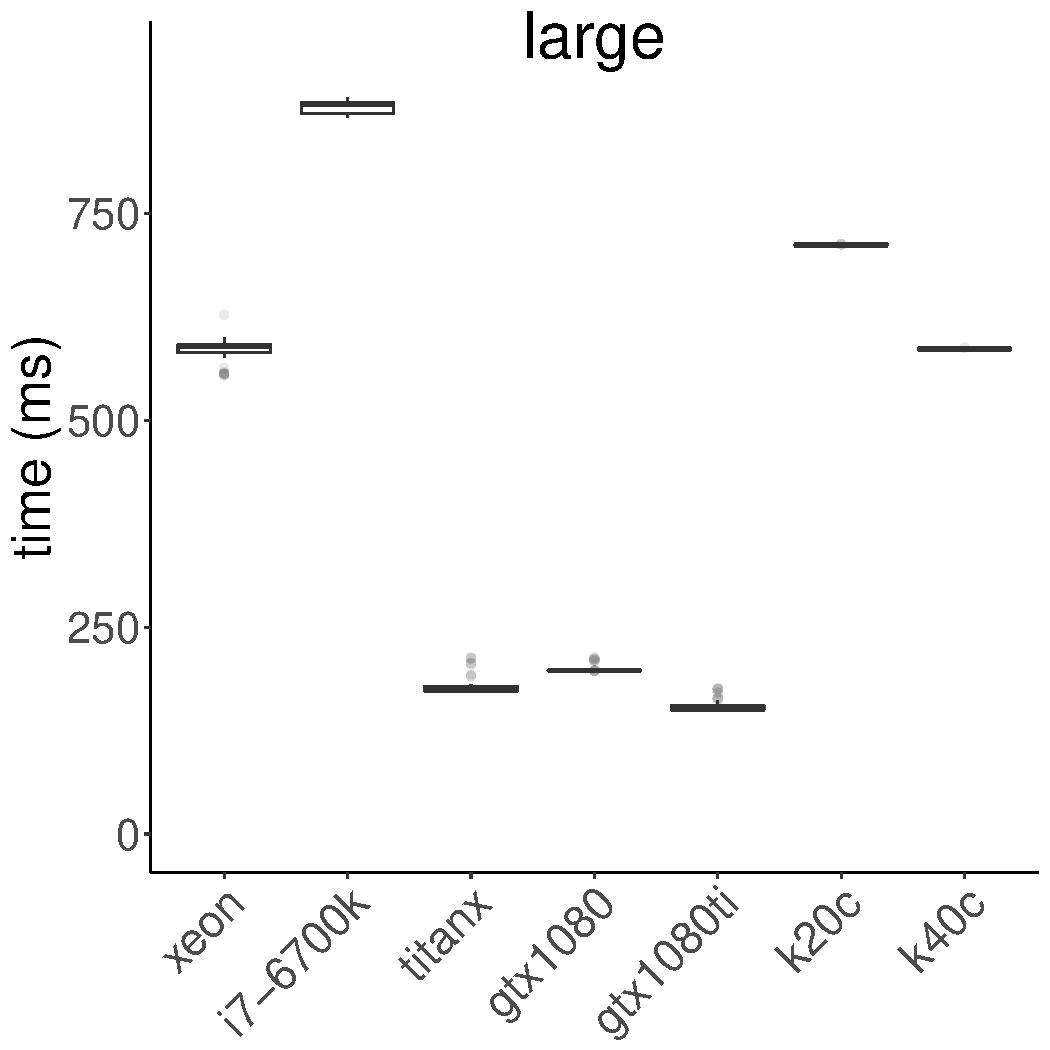
\includegraphics[width=0.22\textwidth]{figures/time-results/generate_lud_large_boxplot-1}
	\end{subfigure}
	
	\begin{subfigure}{0.09\textwidth}\subcaption[l]{\bf dwt} \label{fig:time-dwt} \vspace{5mm}\end{subfigure}
	\begin{subfigure}{0.9\textwidth}
		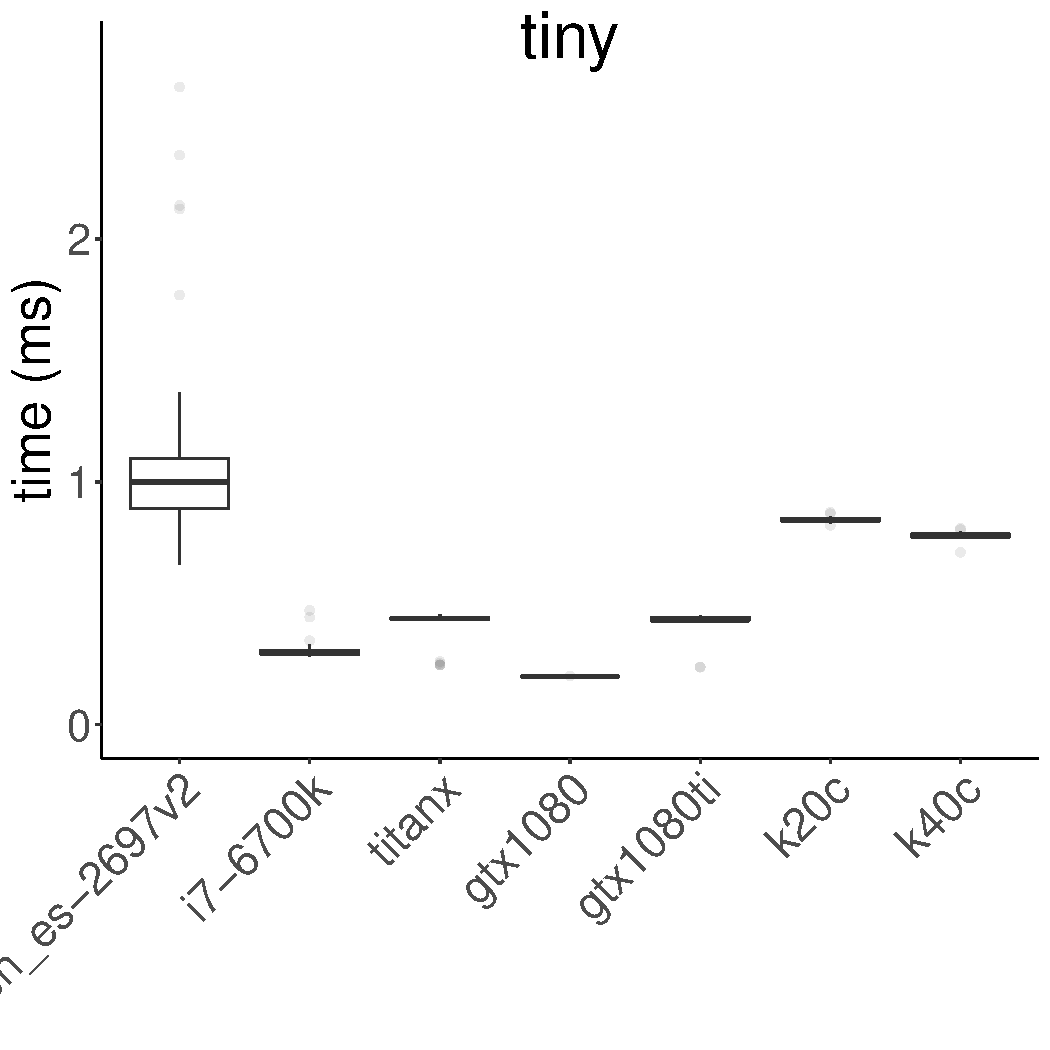
\includegraphics[width=0.22\textwidth]{figures/time-results/generate_dwt_tiny_boxplot-1}
		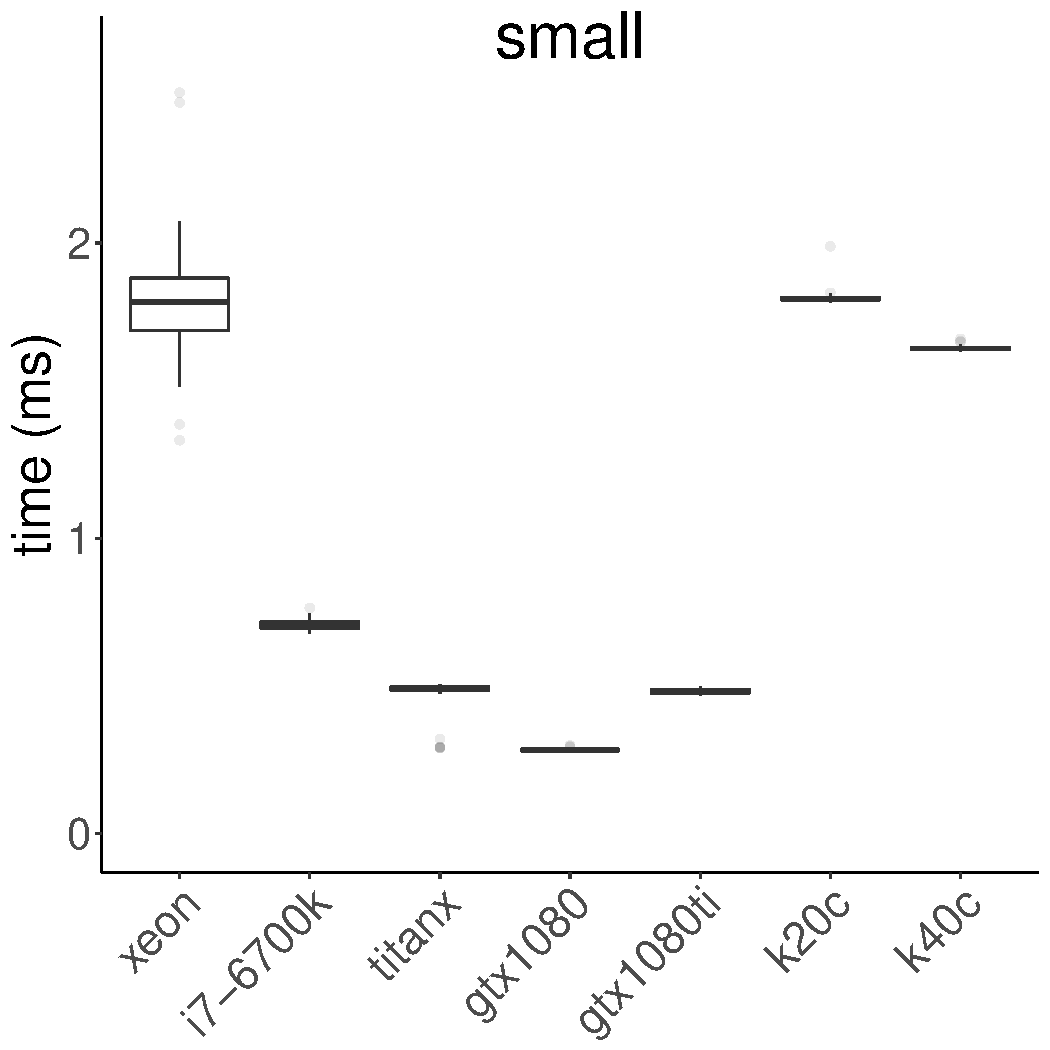
\includegraphics[width=0.22\textwidth]{figures/time-results/generate_dwt_small_boxplot-1}
		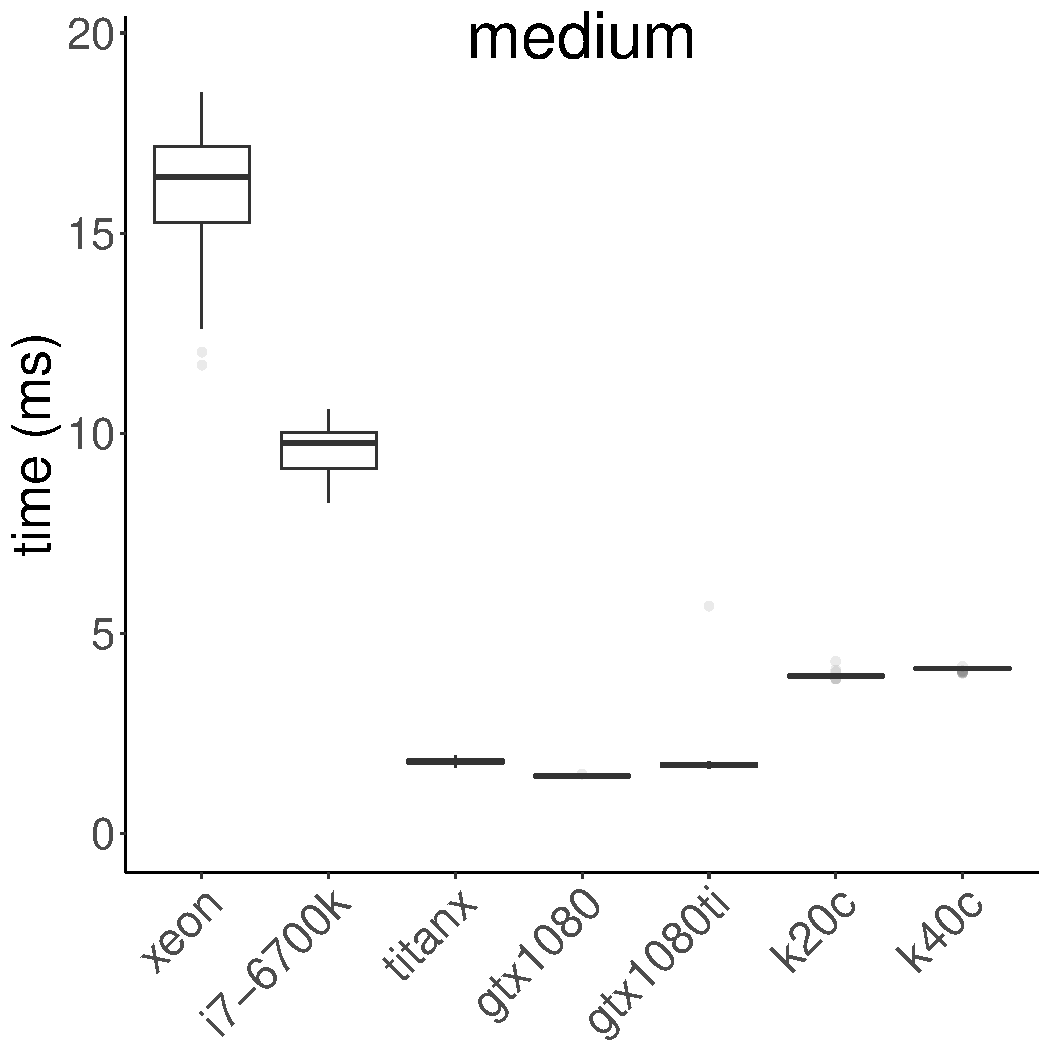
\includegraphics[width=0.22\textwidth]{figures/time-results/generate_dwt_medium_boxplot-1}
		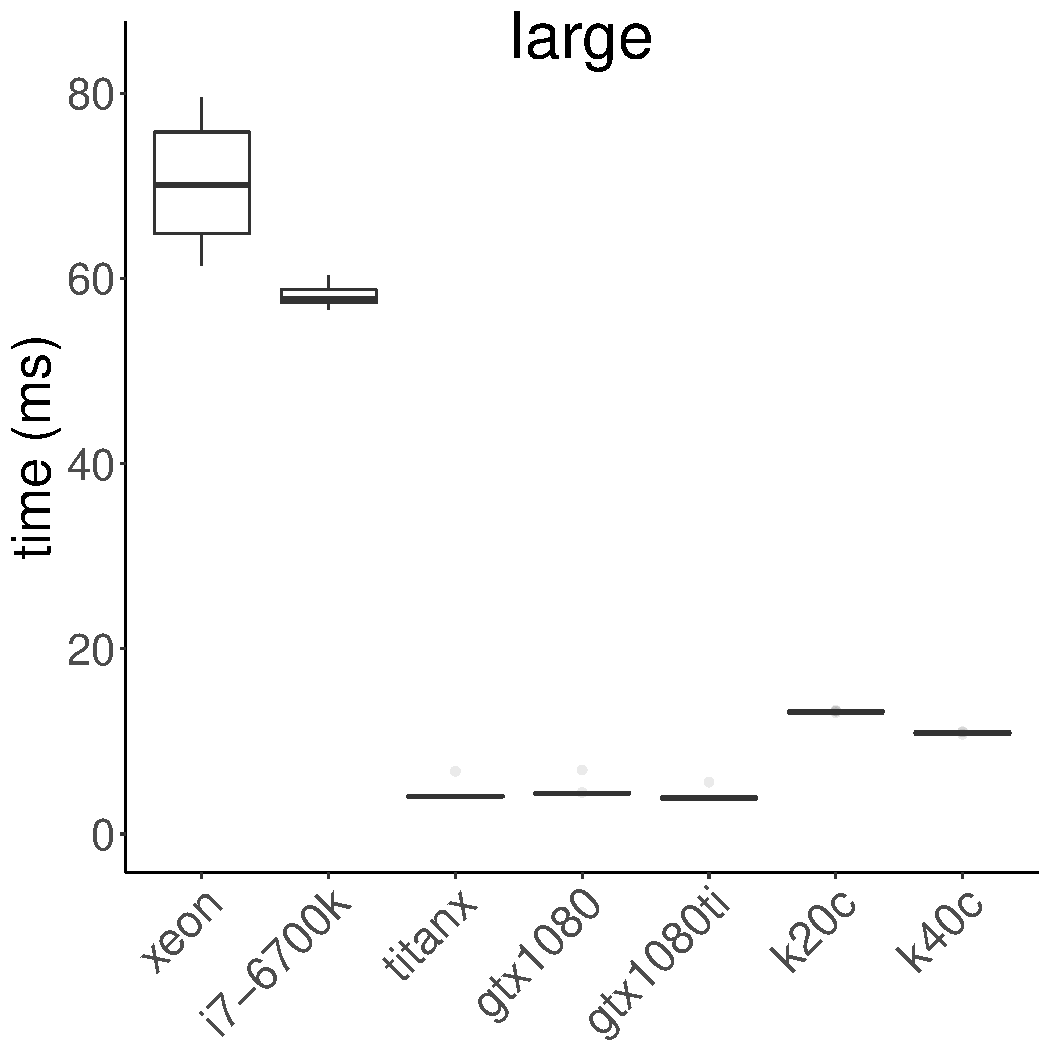
\includegraphics[width=0.22\textwidth]{figures/time-results/generate_dwt_large_boxplot-1}
	\end{subfigure}

	\begin{subfigure}{0.09\textwidth}\subcaption[l]{\bf fft} \label{fig:time-fft} \vspace{5mm}\end{subfigure}
	\begin{subfigure}{0.9\textwidth}
		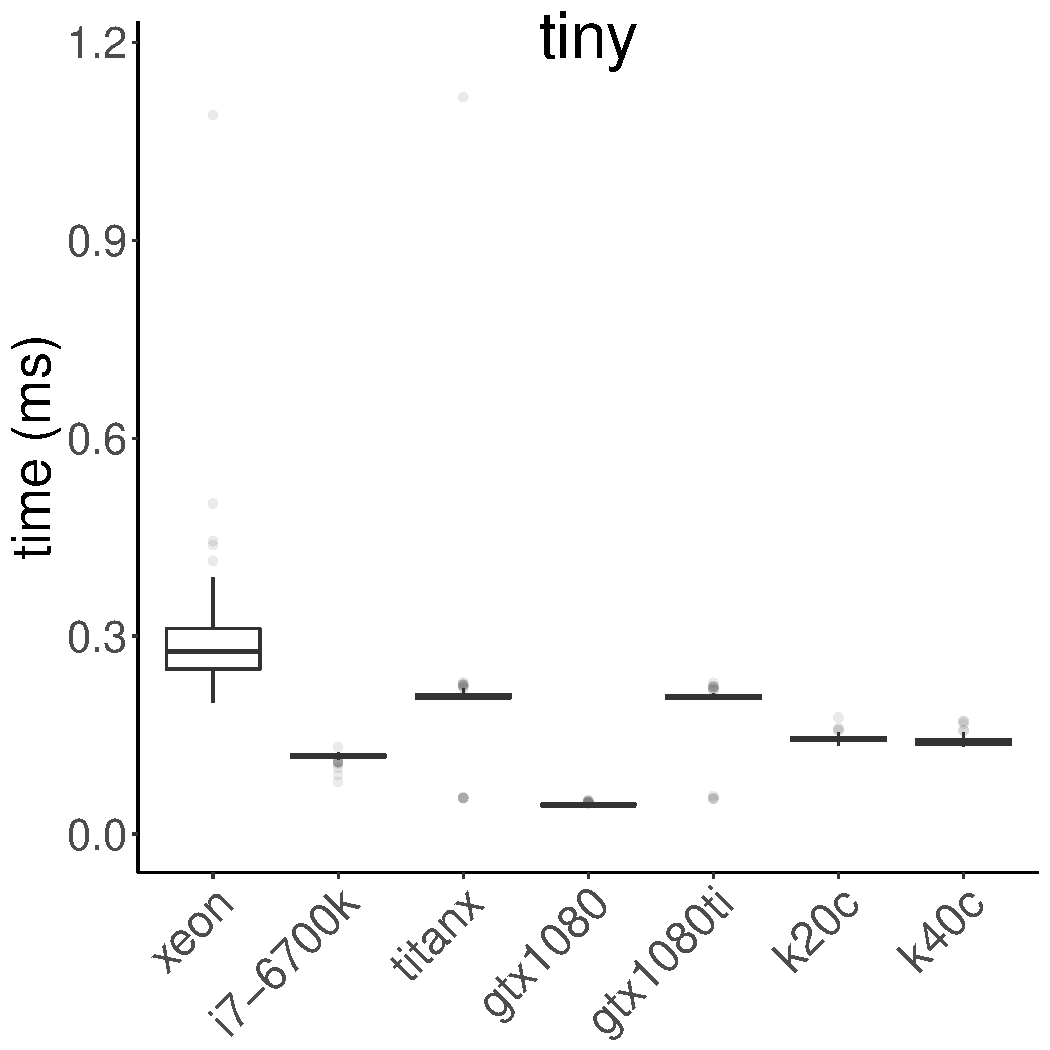
\includegraphics[width=0.22\textwidth]{figures/time-results/generate_fft_tiny_boxplot-1}
		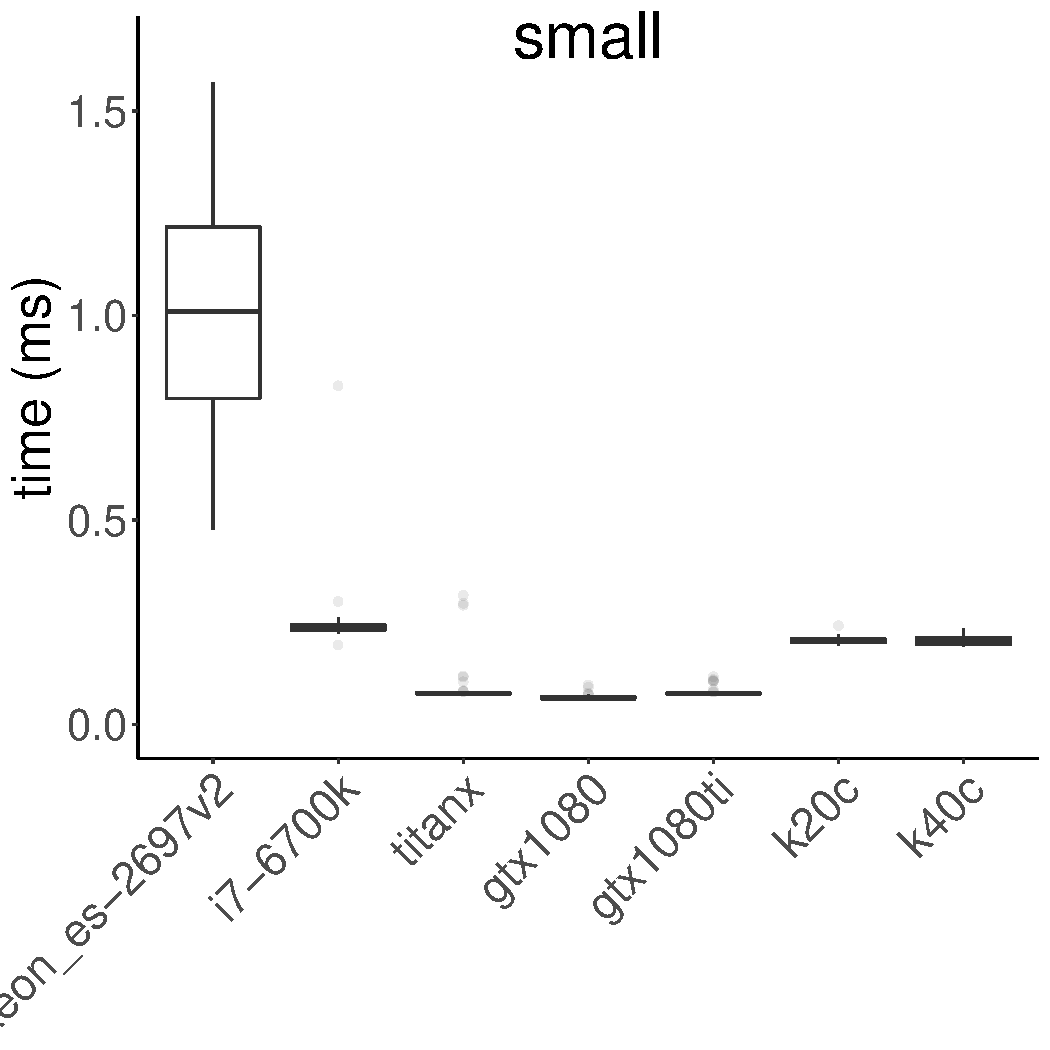
\includegraphics[width=0.22\textwidth]{figures/time-results/generate_fft_small_boxplot-1}
		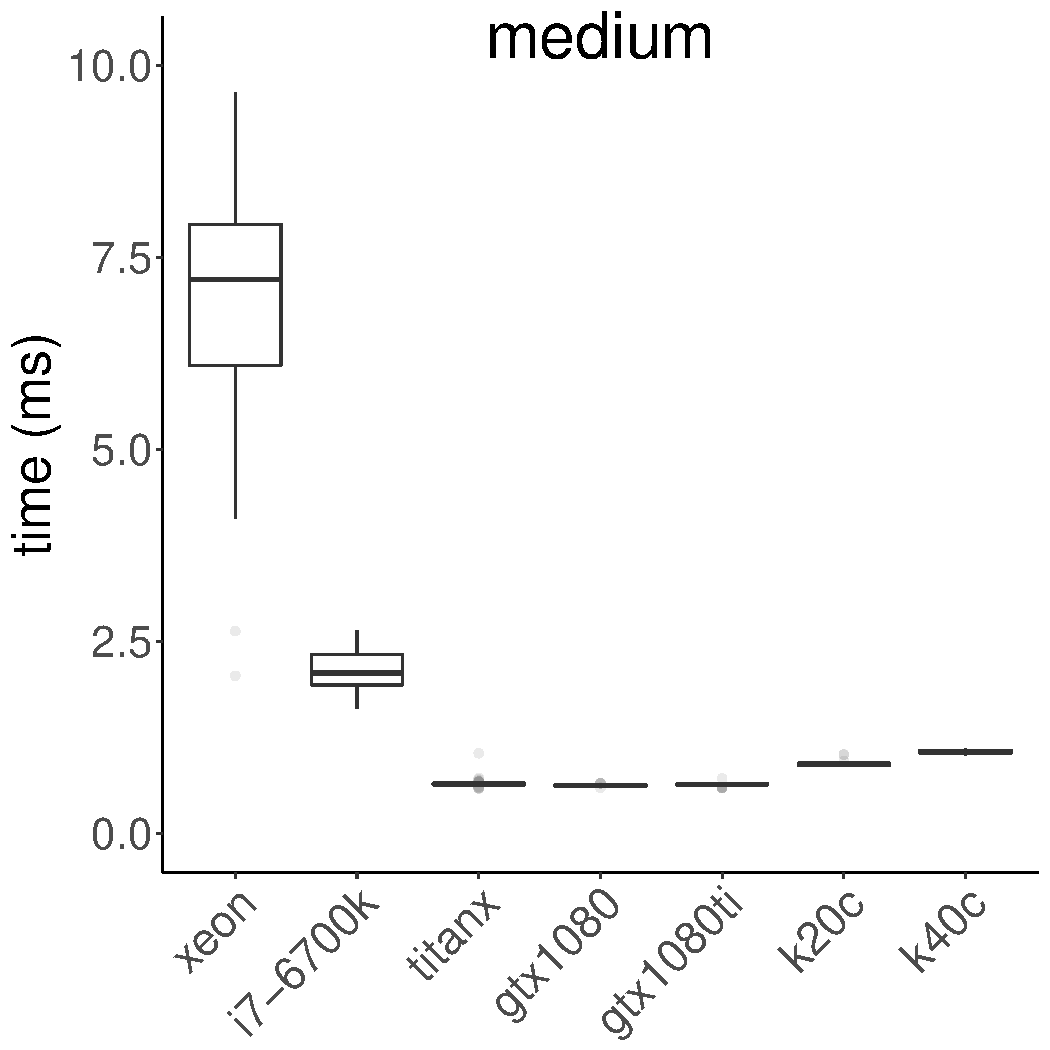
\includegraphics[width=0.22\textwidth]{figures/time-results/generate_fft_medium_boxplot-1}
		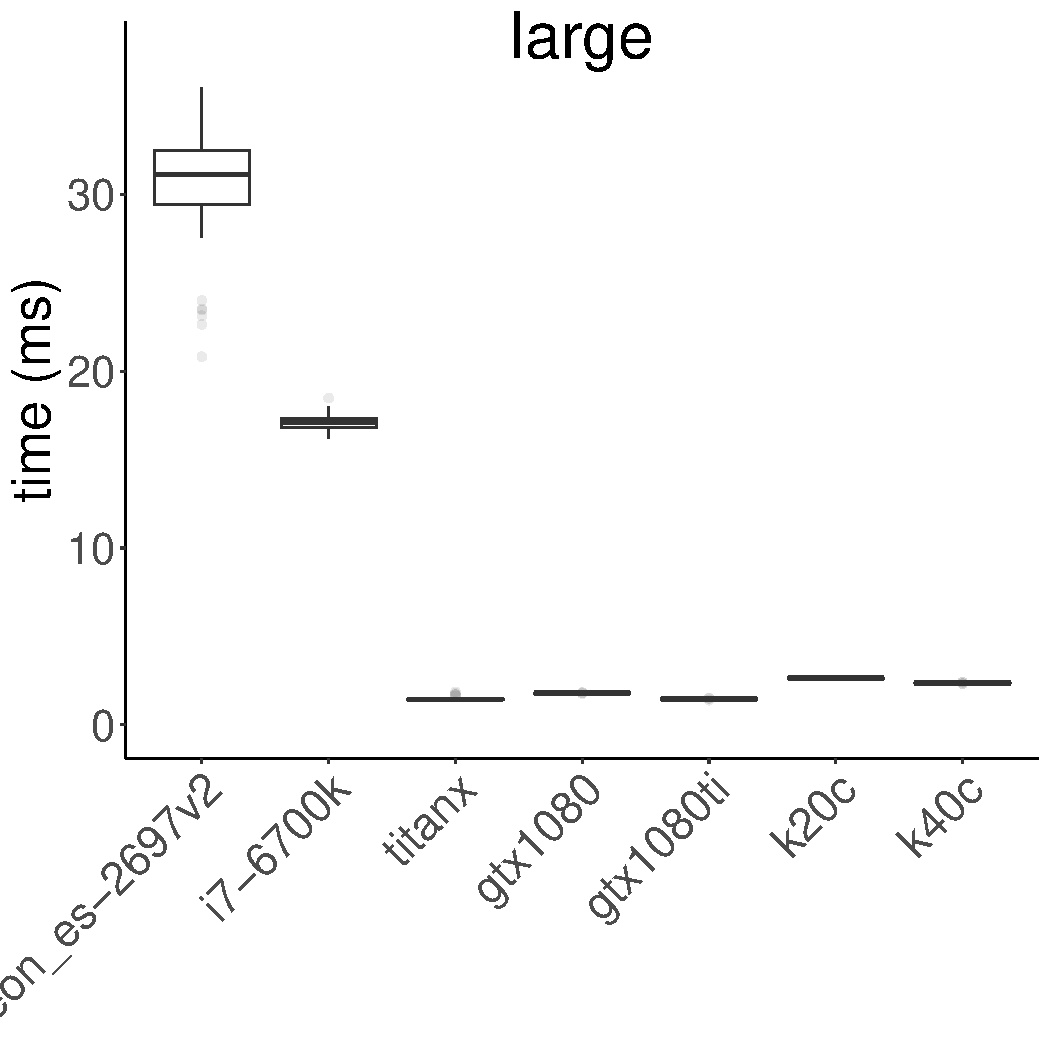
\includegraphics[width=0.22\textwidth]{figures/time-results/generate_fft_large_boxplot-1}
		\end{subfigure}

	\begin{subfigure}{0.09\textwidth}\subcaption[l]{\bf gem} \label{fig:time-gem} \vspace{5mm}\end{subfigure}
	\begin{subfigure}{0.9\textwidth}
		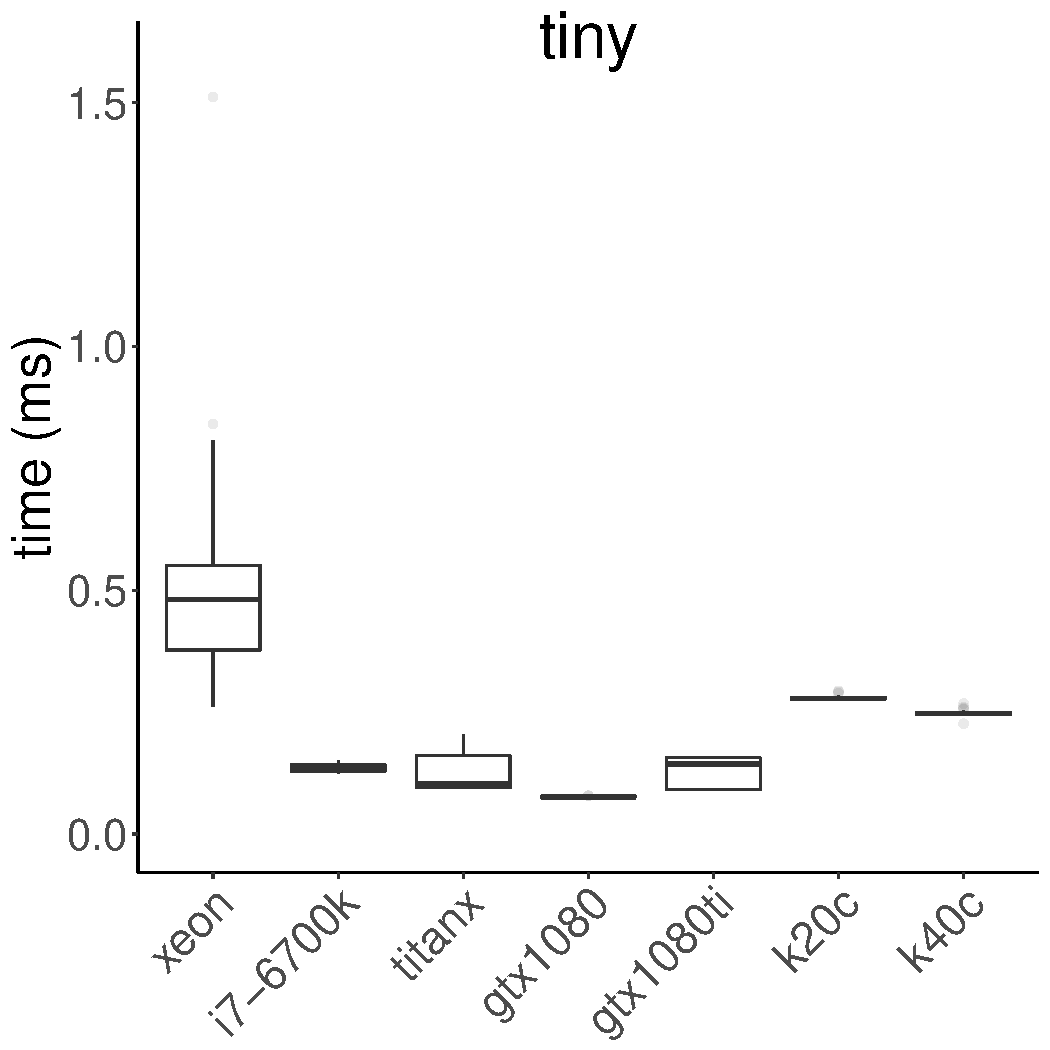
\includegraphics[width=0.22\textwidth]{figures/time-results/generate_gem_tiny_boxplot-1}
		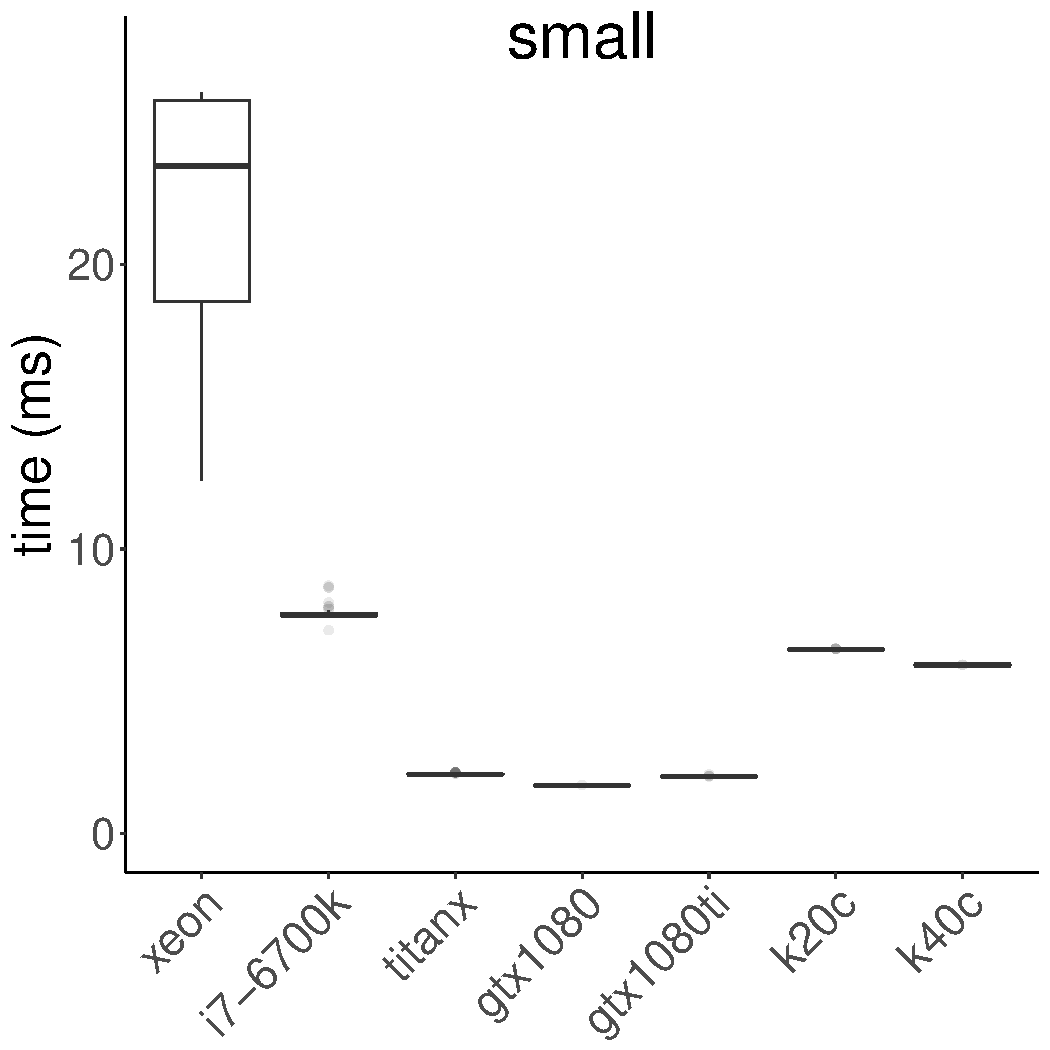
\includegraphics[width=0.22\textwidth]{figures/time-results/generate_gem_small_boxplot-1}
		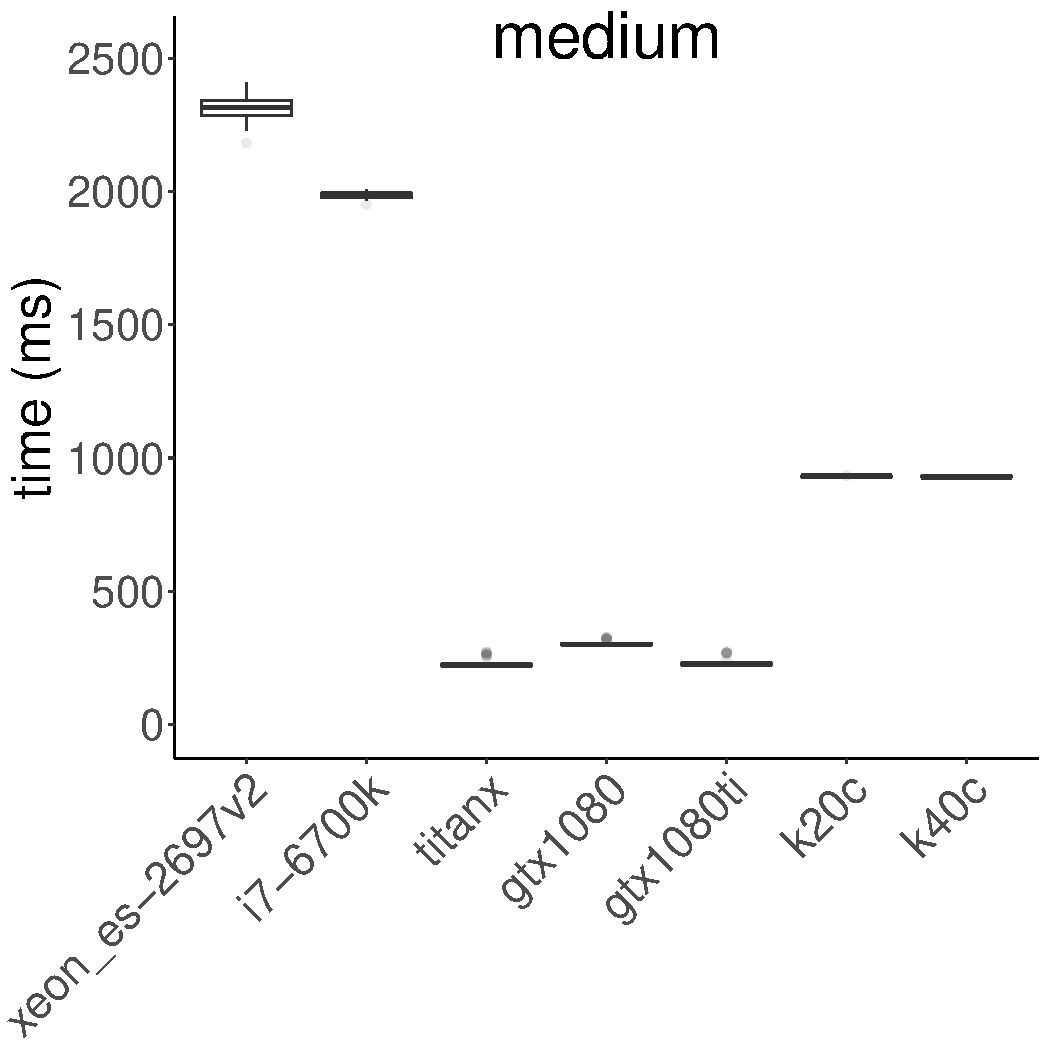
\includegraphics[width=0.22\textwidth]{figures/time-results/generate_gem_medium_boxplot-1}
		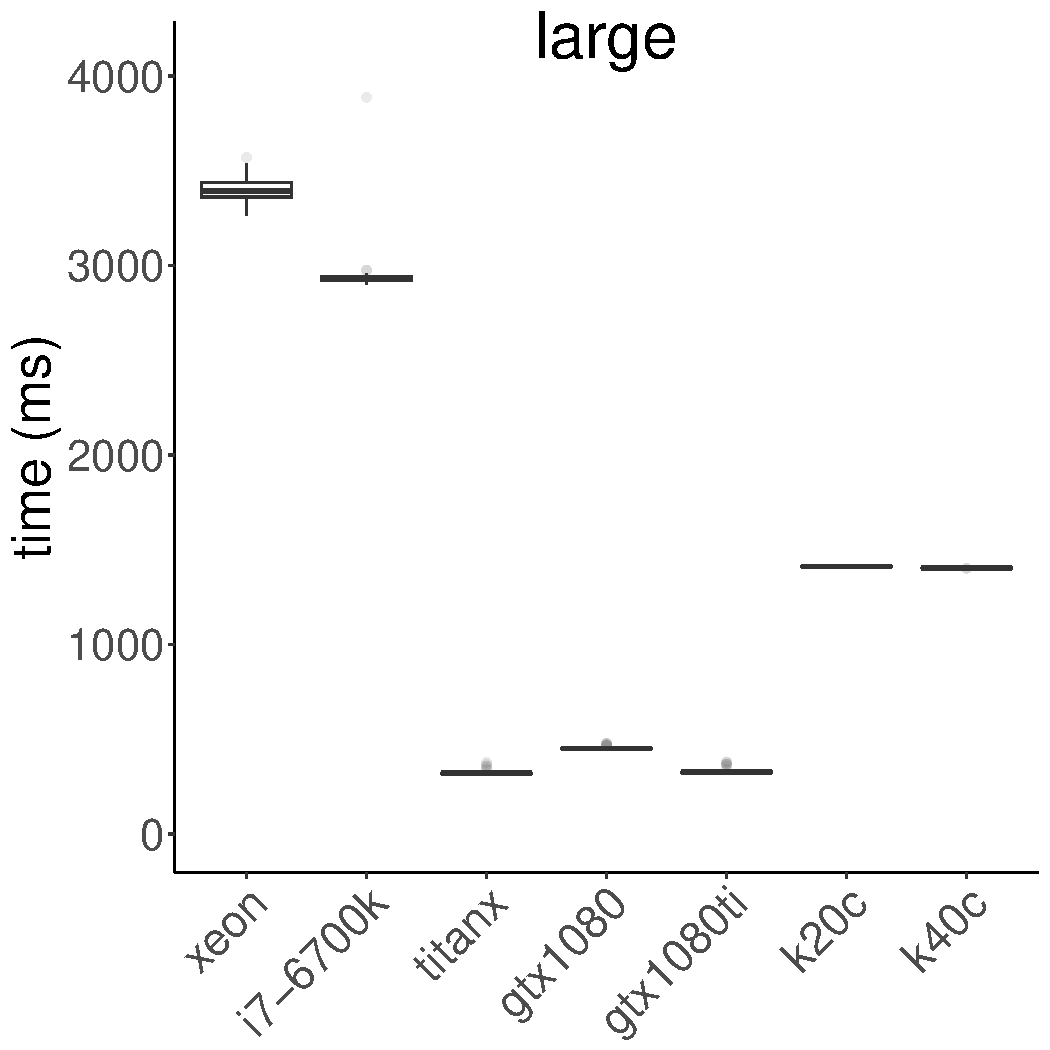
\includegraphics[width=0.22\textwidth]{figures/time-results/generate_gem_large_boxplot-1}
		\end{subfigure}

	\begin{subfigure}{0.09\textwidth}\subcaption[l]{\bf srad} \label{fig:time-srad} \vspace{5mm}\end{subfigure}
	\begin{subfigure}{0.9\textwidth}
		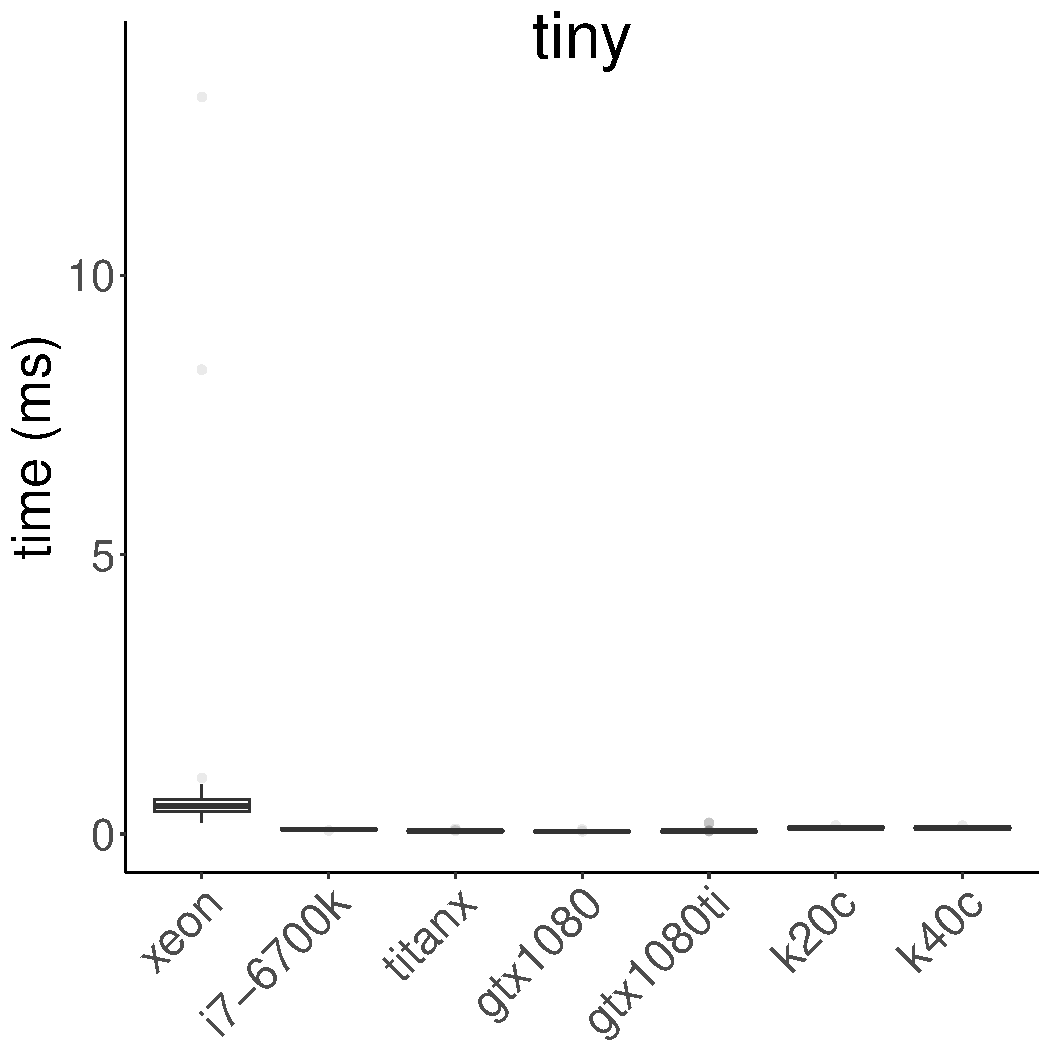
\includegraphics[width=0.22\textwidth]{figures/time-results/generate_srad_tiny_boxplot-1}
		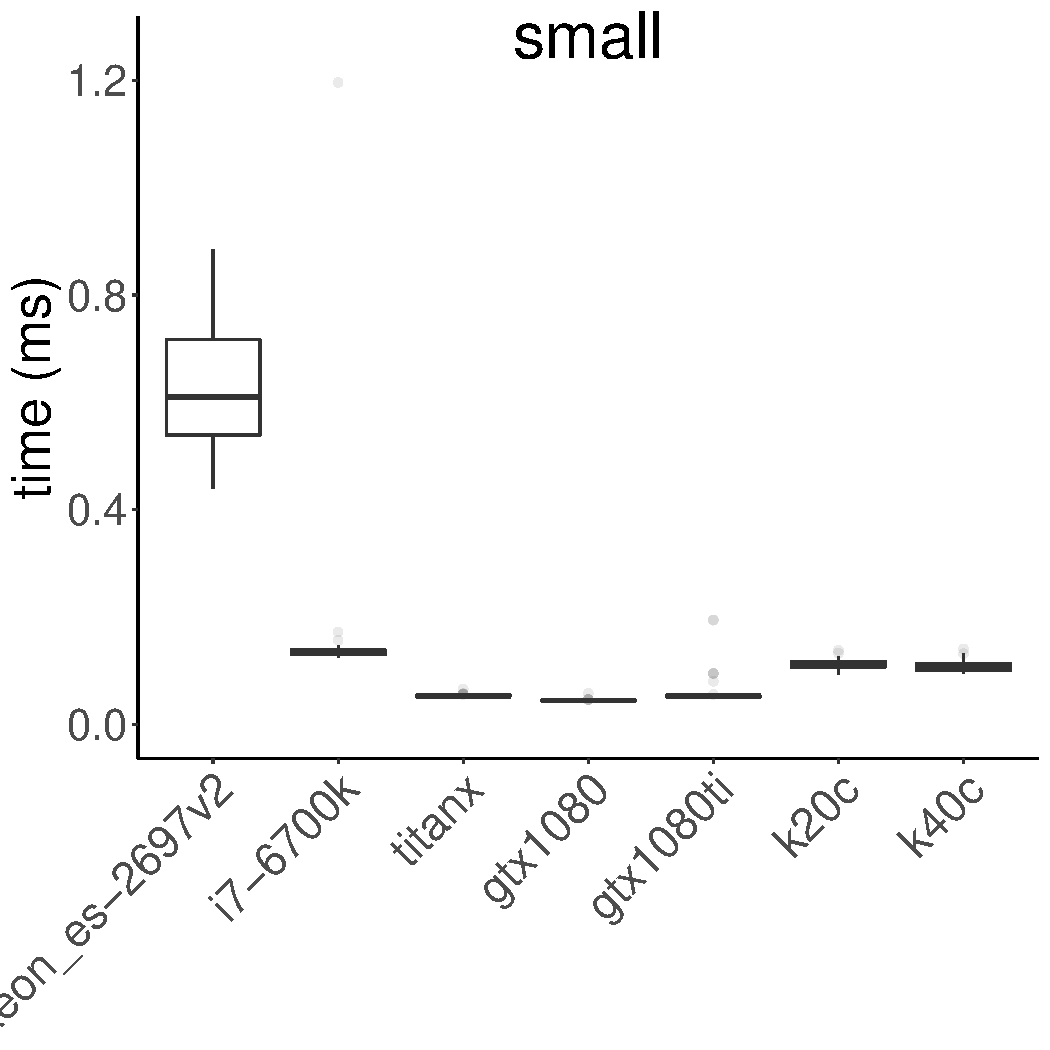
\includegraphics[width=0.22\textwidth]{figures/time-results/generate_srad_small_boxplot-1}
		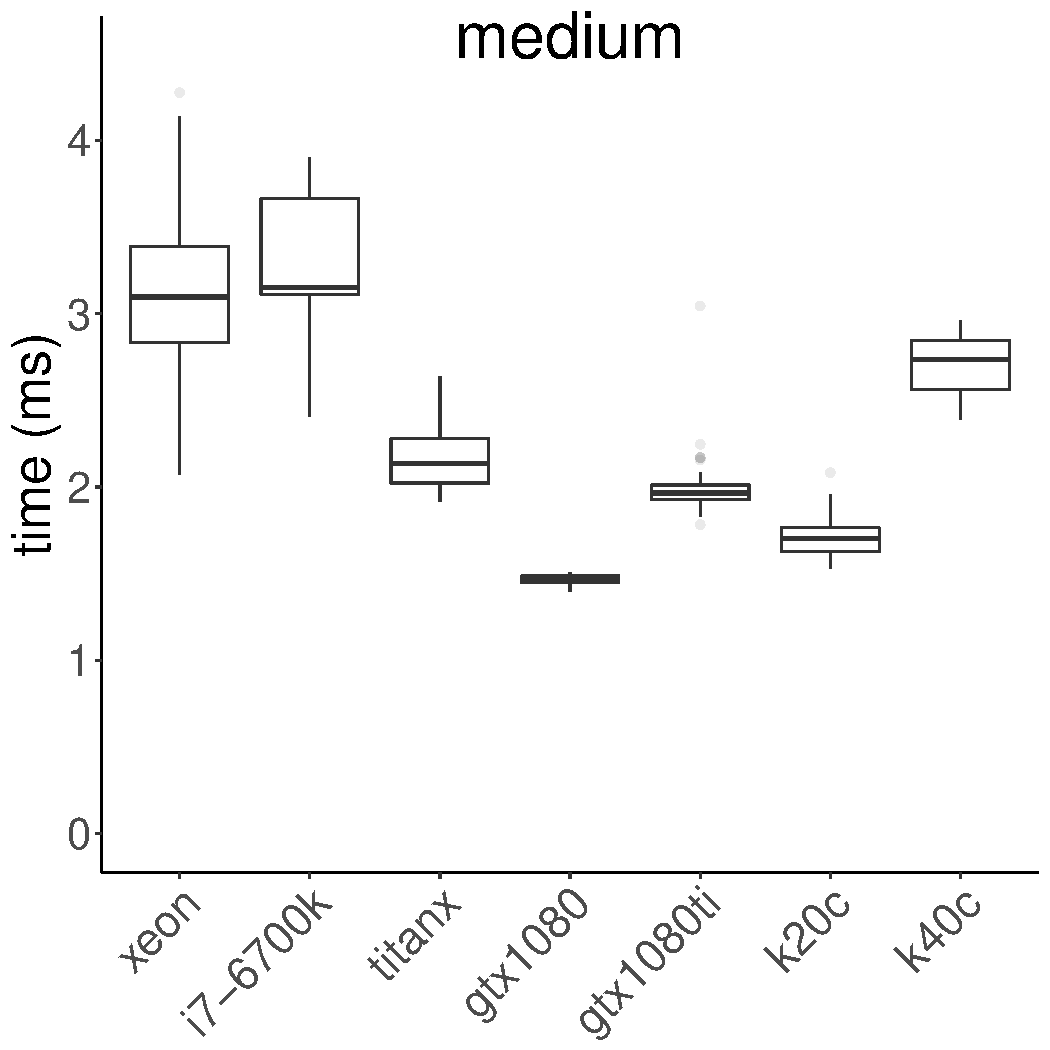
\includegraphics[width=0.22\textwidth]{figures/time-results/generate_srad_medium_boxplot-1}
		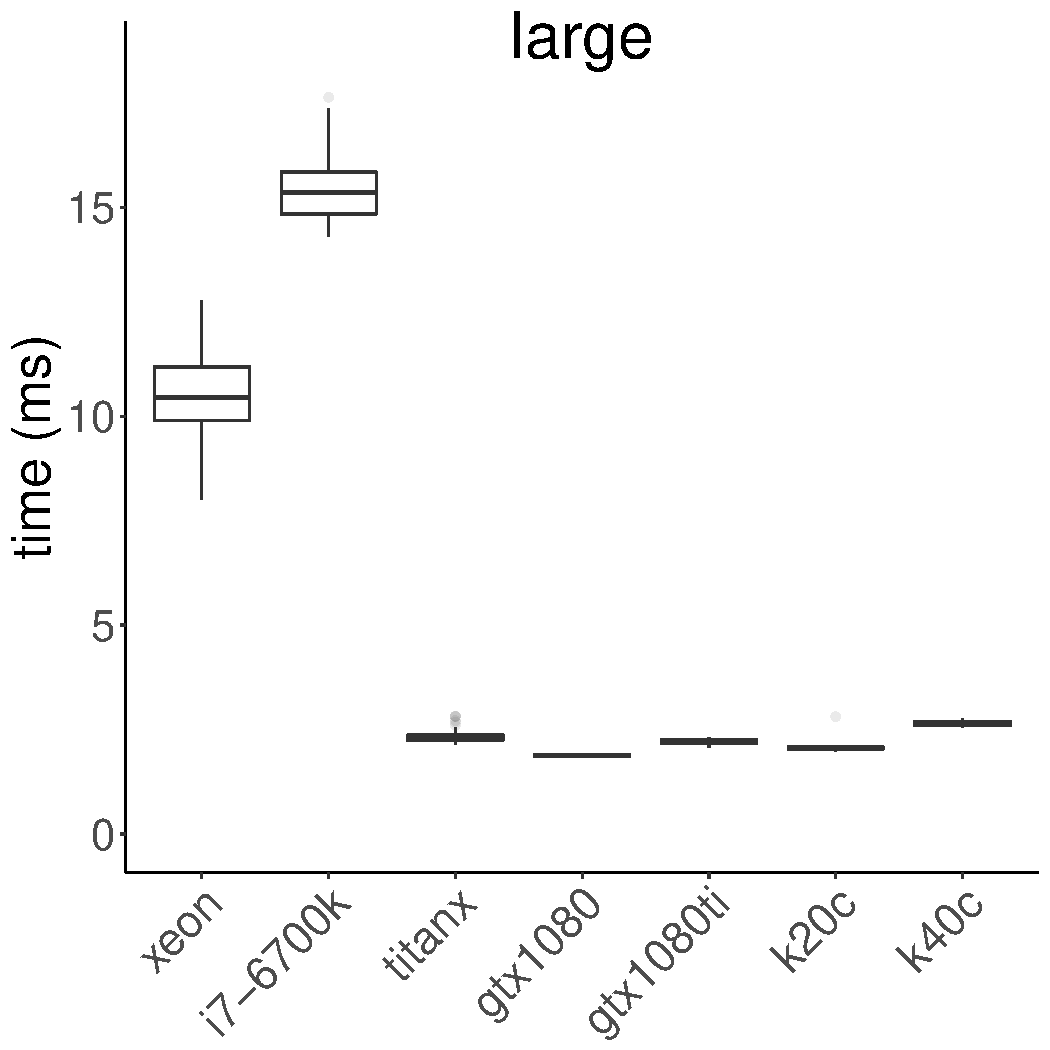
\includegraphics[width=0.22\textwidth]{figures/time-results/generate_srad_large_boxplot-1}
	\end{subfigure}
    \caption{Kernel execution times for benchmarks for which the GPU architectures are optimal}\label{fig:time}
\end{figure*}


Figure~\ref{fig:time} shows the distribution of execution times for each benchmark over 50 iterations.
LibSciBench has a high resolution timer with one cycle resolution and roughly \SI{6}{\nano\second} of overhead.

Each benchmark corresponds to a particular dwarf, for instance Figure~\ref{fig:time-kmeans} and Figure~\ref{fig:time-lud} are both representative of the Dense Linear Algebra dwarf, whereas Figure~\ref{fig:time-dwt} and Figure~\ref{fig:time-fft} are representative of Spectral Methods.
Figure~\ref{fig:time-gem} represents N-Body Methods, Figure~\ref{fig:time-srad} encompasses a Structured Grid Method of Dwarf, and finally Figure~\ref{fig:time-crc} is a problem from Combinational Logic.
All but the {\bf crc} benchmark perform best on GPU type accelerators.

\todo{Are there any benchmarks where increasing the problem sizes makes results worse for the GPU?}
\todo{How does changing problem sizes affect benchmark performance across a range of platforms (selected accordingly to cache size)?}
\todo{Comment on the similarities within a dwarf and the differences between them.}

\end{document}
